\documentclass{IEEEtran}

\usepackage{graphicx}
\usepackage{hyperref}

\title{A mutual information based medical image registration methodology based on JVHW entropy estimator}
\author{Sihan Li, Tsinghua University}

\begin{document}
  \maketitle

  \begin{abstract}
    Mutual information (MI) based medical image registration has gained much attention for its robustness. However, Jiao found that maximum likelihood estimator (MLE), although widely used to implement MI-based registration, is sub-optimal when the number of observations is comparable to the parameter dimension \cite{jiao2015minimax}. They proposed a new entropy estimator, JVHW estimator, which is claimed to outperform MLE estimator. Based on previous works, we propose a mutual information based registration methodology based on JVHW entropy estimator. The contribution of this paper can be divided into three parts: 1) A C++ version of JVHW estimators using only C++ standard library is effectively implemented, 2) a new similarity metric based on JVHW mutual information estimator is created as an elastix component, and 3) the new metric is evaluated and compared with other metrics. Dataset from Retrospective Image Registration Evaluation Project (RIRE) is used to evaluate and compare various implementations.

  \end{abstract}

  \section{Introduction}

  Image registration is a process of aligning two or more images geometrically. These images can be taken at different time, from different viewpoints or from different sensors. It is vital in image analysis when the data collected from different sources need to be combined. To achieve this, a variety of techniques have been developed and researched, aiming for different kinds of applications. \cite{brown1992survey, zitova2003image}

  Image registration methodologies consist of three major parts: \emph{Similarity measures}, which measure the degree of similarity between two images. \emph{Transforms}, which transform pixels/voxels from one image domain to another. \emph{Optimizations}, which minimize the similarity measures to achieve the registration.

  Similarity measure is a criteria to judge the degree of similarity of two images. It is know as \emph{cost function}, or \emph{registration basis} in Maintz's classification \cite{maintz1998survey}. Commonly used measures include intensity based measures, which analysis the images as a whole, and feature based measures, which detect and match features of two images.

  \subsection{Mutual information}

  Mutual information based registration methodologies use mutual information (MI) or its variant as the similarity measures. It is a kind of area-based metric. The Methodology based on a simple assumption that the gray level distributions of images to be registered are correlated. Mutual information is defined as:

  \begin{equation}
    I(A, B) = H(A) + H(B) - H(A, B)
  \end{equation}

  where $H(A)$ is the entropy of $A$. It describes the amount of uncertainty about image minus the uncertainty about $A$ when $B$ is known \cite{pluim2003mutual}. The most common entropy measure used in paper is Shannon entropy, which is defined as

  \begin{equation}
    H = -\sum_i{p_i\log{p_i}}
  \end{equation}

  where $p_i$ represents the probability of a event $e_i$. In order to register two images, the joint gray value distribution is calculated from them. Other entropy measures include Arimoto entropy \cite{li20153d}, Tsallis entropy \cite{khader2012information} etc.

  A popular variant of MI is Normalized mutual information (NMI), which is overlap invariant, which is defined as

  \begin{equation}
    NMI(A, B) = \frac{H(A) + H(B)}{H(A, B)}
  \end{equation}

  by Studholme in 1999 \cite{studholme1999overlap}. To achieve image registration, the MI/NMI between two images are maximized. Mutual information based measures are generally applicable, and does not need complex initialization \cite{pluim2003mutual}.


  % \subsection{Retrospective Image Registration Evaluation Project}

  % Retrospective Image Registration Evaluation Project (RIRE) is a project designed to compare different registration techniques. It contains a set of CT, PET and MR images. An example of the input images is shown in Figure~\ref{fig:before-registration}. Each MR-CT images pair and MR-PET images pair has been corrected using frames and markers, so the results of different registration methods can be compared with the ``gold standard'' registration results.

  % In RIRE dataset, a ``from'' image, which is a CT or PET image, is registered to a ``to'' image, which is a MR image. The relation is depicted in Figure~\ref{fig:RIRE-from-to}. An example of an image pair can be seen in Figure~\ref{fig:before-registration}. The transformations are expected to be rigid, and can be uploaded to compare with the ``gold standard'' transformations. The transformation is described by the transformed coordinates of eight corner in moving image. We are using RIRE to measure the performance of different registration methodologies.

  % \begin{figure}[htbp]
  %   \centering
  %   \includegraphics[width=0.7\columnwidth]{RIRE_from_to.jpg}
  %   \caption{Modalities of images in RIRE project. The registration is expected to be done from left (CT/PET) to right (different weighted MR). \cite{rireprotocol}}
  %   \label{fig:RIRE-from-to}
  % \end{figure}

  % \begin{figure}[htbp]
  %   \includegraphics[width=\columnwidth]{before_registration.png}
  %   \caption{A CT(green layer)-MR(red layer) image pair from RIRE project. Notice the two images are different in size.}
  %   \label{fig:before-registration}
  % \end{figure}

  \subsection{JVHW estimators}

  As we mentioned before, MI-based methodologies calculate the mutual information between two gray level distributions. However, in reality the distributions are unknown, so the exact MI can not be calculated and needs to be estimated. Most implementations simply use a straightforward maximum likelihood estimator (MLE) to estimate MI. However, Jiao pointed out that MLE and other previous prevailing approaches can be highly sub-optimal, and proposed a \emph{minimax} entropy/MI estimator, which means the estimator minimizes the maximum $L_2$ risk \cite{jiao2015minimax}. They showed that their estimator outperform MLE and many other estimators.

  \section{Implementations}

  \subsection{C++ version of JVHW estimator}

  In order to make a comparison between MLE and JVHW estimator, we are going to re-implement both of them in C++. To reuse as much as code as possible, we have to analyze both estimator and point out what they have in common. Actually, both of the estimator are linear estimators which can be expressed in the following way:

  \begin{equation}
    H = \sum_{i = 1}^n{a_jF_j},
  \end{equation}

  Where $F_j$ is called ``fingerprint'', representing the number of symbols that show up for $j$ times in the sample. The only different between two estimator is $a_j$. In MLE it follows the following form:

  \begin{equation}
    a_j = -\frac{j}{n}\log_2{\frac{j}{n}},
  \end{equation}

  and in JVHW estimator $a_j$ is calculated during run time. So instead of simply migrating MATLAB or Python code into C++ code, we divide the function into several sub-function. That is:

  \subsubsection{CalculateFingerprint}
  Collect the samples into a certain number of bins to get a histogram, then calculate the fingerprint from it.

  \subsubsection{est\_entro\_JVHW}
  Estimator entropy from an integer vector using JVHW estimator.

  \subsubsection{est\_entro\_MLE}
  The same as above, except using MLE.

  \subsubsection{NormalizeVector}
  Normalize the sample from a double vector to an integer vector.

  \subsubsection{CombineVector}
  Combine samples to form a joint-distributed sample.

  \subsubsection{est\_MI\_JVHW}
  Invoke above functions to calculate the MI.

  \subsubsection{est\_MI\_MLE}
  The same as above, except using MLE.


  To avoid file operations which will take lots of time, we embed \texttt{poly\_coeff\_r} into our source code. That is, we make it a static array, which will be loaded into the memory only once when the program starts. It will take about 314 KB memory. Given that metric function will be invoked continuously during registration, this memory consumption is really acceptable.

  \subsection{Elastix component}

  Elastix is built using CMake, and has been divided into small components. In order to add new metrics, optimizers, transformations or something else into elastix, one has to:

  \begin{enumerate}
    \item Implement an \texttt{itk} class, which does the actual works.
    \item Implement an \texttt{elastix} class, which takes care of things like parameter-setting.
    \item Put source files in the correct directory together with a \texttt{CMakeLists.txt}, which declares the component.
    \item Re-compile elastix.
  \end{enumerate}

  So in order to use JVHW entropy estimator in the metric, we have to implement two classes. Building the classes from nowhere can be a painful and error-prone, so we take most of the code from \texttt{AdvancedMeanSquares}, which is a simple metric that iterate over every voxels and compute the mean square error.

  \subsection{Optimizers and parameters}

  Elastix offers a branch of built-in optimizers, including \emph{Adaptive Stochastic Gradient Descent}, \emph{Standard Gradient Descent}, \emph{Quasi Newton LBFGS} etc. However, it should be noticed that most of the optimizers need to know the derivative of the cost function, which is especially hard to acquire when applying JVHW entropy estimator. Therefore, we will pick our optimizer from the ones that do not need to know the derivative of the cost function. Both \emph{CMA Evolution Strategy} and \emph{Simultaneous Perturbation} has been tested, and the latter one shows more robustness when applied to our problem.

  When it comes to parameters, \emph{Maximum Number Of Iterations} has been set to 500.

  The source code is available at \url{https://github.com/ThomasLee969/stanford-project}.

  \section{Results}

  To evaluate the two new metrics, we have to make sure that they are valid metric, and can be used to preform image registration. Thus, we perform registration on RIRE dataset using four metrics: \emph{Mattes MI}, \emph{NMI}, \emph{MLE} and \emph{JVHW}. The former two metrics are shipped with elastix. They use \emph{Parzen window method}, also known as \emph{kernel density estimate method}, to estimate the underlying distribution from a series of samples, as depicted in Figure~\ref{fig:parzenhistogram}

  \begin{figure}[htbp]
    \centering
    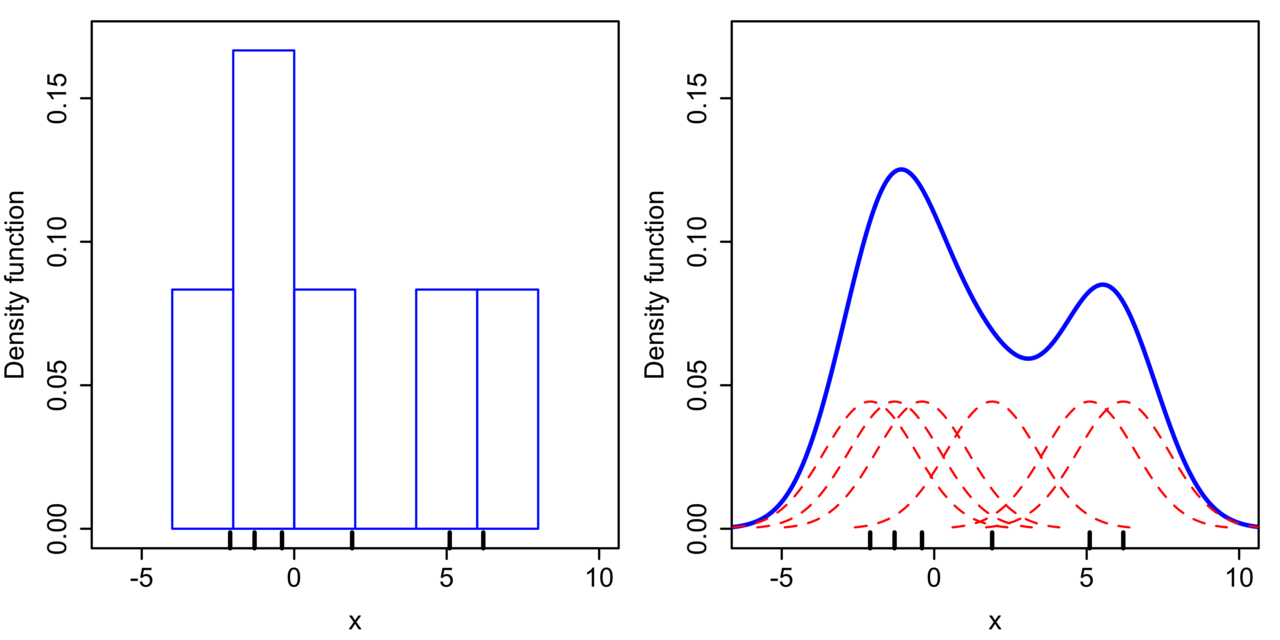
\includegraphics[width=\columnwidth]{parzenhistogram.png}
    \caption{Comparison of a histogram and a kernel density estimate.}
    \label{fig:parzenhistogram}
  \end{figure}

  Also, for \emph{Mattes MI}, \emph{NMI} method we also deploy a \emph{Adaptive Stochastic Gradient Descent} optimizer. The result can be seen in Figure~\ref{fig:CT_32bin} and Figure~\ref{fig:PET_32bin}

  \begin{figure}[htbp]
    \centering
    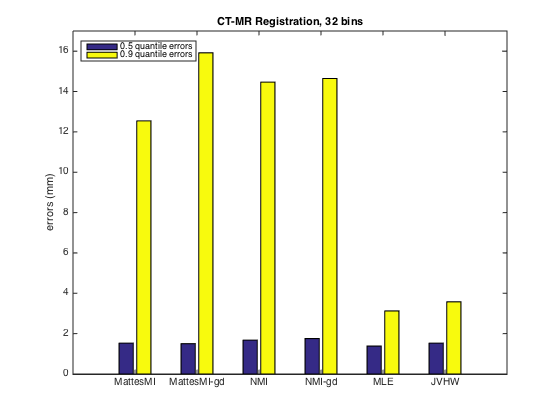
\includegraphics[width=\columnwidth]{CT_32bin.png}
    \caption{Quantile errors for CT to MR registration using 32 bins.}
    \label{fig:CT_32bin}
  \end{figure}

  \begin{figure}[htbp]
    \centering
    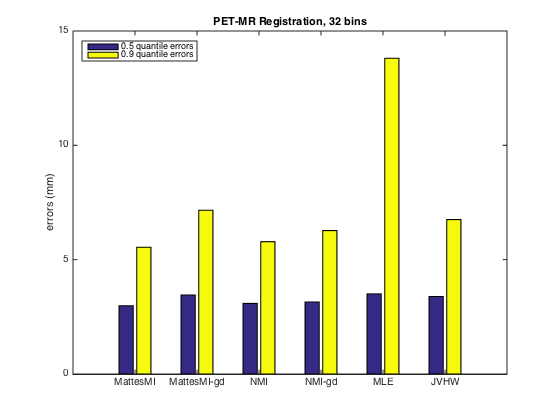
\includegraphics[width=\columnwidth]{PET_32bin.png}
    \caption{Quantile errors for PET to MR registration using 32 bins.}
    \label{fig:PET_32bin}
  \end{figure}

  We adopt the methodologies using in \cite{pluim2004f} to evaluate the accuracy of each implementation. The 0.5 and 0.9 quantile errors over all CT-MR and PET-MR pairs of 9 patients have been calculated. 0.9 quantile is used instead of the maximum value, because the maximum can be affected by a single outliers. It can be seen that we have implemented our metrics correctly. Moreover, our metrics outperform the built-in MI-based metrics.

  Having confirmed that we have implemented the metrics correctly, we are going to adjust the number of bins, which is one of the most important parameters in our metrics. The results can be seen in Figure~\ref{fig:CT-MLE-JVHW} and Figure~\ref{fig:PET-MLE-JVHW}.

  \begin{figure}[htbp]
    \centering
    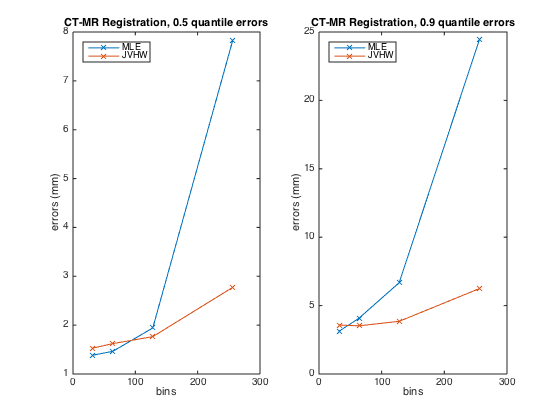
\includegraphics[width=\columnwidth]{CT-MLE-JVHW.png}
    \caption{Quantile errors for CT to MR registration}
    \label{fig:CT-MLE-JVHW}
  \end{figure}

  \begin{figure}[htbp]
    \centering
    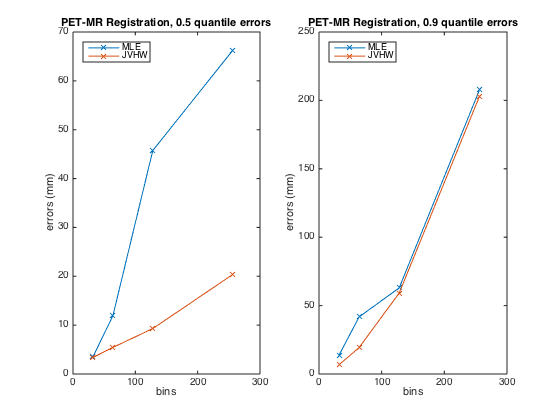
\includegraphics[width=\columnwidth]{PET-MLE-JVHW.png}
    \caption{Quantile errors for PET to MR registration}
    \label{fig:PET-MLE-JVHW}
  \end{figure}

  It can be seen that when there are few bins, MLE performs a little bit better than JVHW. But when the number of bins increase, the errors given by MLE increase faster than the errors given by JVHW. This is because when the number of samples is significantly larger than the support size, the MLE is essentially the optimal scheme. In our situation, the support size is about $10^3$, while the number of samples is about $10^6$. So it can be concluded that our JVHW-based metric outperform traditional MLE metric in general, especially when the number of bins are large.

  \section{Acknowledgment}

  The images and the standard transformation(s) were provided as part of the project, ``Retrospective Image Registration Evaluation'', National Institutes of Health, Project Number 8R01EB002124-03, Principal Investigator, J. Michael Fitzpatrick, Vanderbilt University, Nashville, TN.

  \bibliographystyle{IEEEtran}
  \bibliography{task4}

\end{document}
